\documentclass[12pt]{article}

\usepackage{geometry}
\usepackage{indentfirst}
\usepackage{fancyhdr}
\usepackage{graphicx}
\usepackage{amsmath}
\usepackage{amsthm}
\usepackage{amssymb}
\usepackage{mathtools}
\usepackage{xcolor}
\usepackage{listings}
\usepackage{hyperref}

\newcommand{\Team}{IMMC23413340}
\newcommand{\Title}{How to distinguish biological species by numbers?}

\definecolor{codegreen}{rgb}{0,0.6,0}
\definecolor{codegray}{rgb}{0.5,0.5,0.5}
\definecolor{codepurple}{rgb}{0.58,0,0.82}
\definecolor{backcolour}{rgb}{0.95,0.95,0.92}

\lstdefinestyle{mystyle}{
    backgroundcolor=\color{backcolour},   
    commentstyle=\color{codegreen},
    keywordstyle=\color{magenta},
    numberstyle=\tiny\color{codegray},
    stringstyle=\color{codepurple},
    basicstyle=\ttfamily\footnotesize,
    breakatwhitespace=false,         
    breaklines=true,                 
    captionpos=b,                    
    keepspaces=true,                 
    numbers=left,                    
    numbersep=5pt,                  
    showspaces=false,                
    showstringspaces=false,
    showtabs=false,                  
    tabsize=2
}

\lstset{style=mystyle}

\title{IMMC GC 2023 Winter\\ Problem E}
\author{Team\#\Team}

\graphicspath{{./figures}}

\pagestyle{fancy}
\fancyhead[R]{\Team}
\fancyhead[L]{Page \thepage \ of 15}

\setlength{\parindent}{20pt}

\newtheorem{lemma}{Lemma}
\newtheorem{corollary}{Corollary}
\newtheorem{classifier}{Classifier}

\begin{document}
\maketitle
\begin{center}
\rule{13cm}{0.4pt}
\end{center}
\thispagestyle{empty}

\begin{center}
\section*{Abstract}
\end{center}

Biological classification is a basic method for studying organisms based on morphological characteristics and physiological functions, which is conducive to the protection of ecological diversity.  For the past decades, with the development of science and technology, people have achieved higher attainments in the field of biological classification. This article aims to establish standards to help biologists to analyse lizards more conveniently which have different appearances when the characteristic attributes of lizards are known.

Firstly, we plotted out the feature histogram with regard to the
species of lizards, to have a basic understanding to the data.
By the histogram, we find out that the FNPr value of most
lizard species 5 is far smaller than others. Afterwards, we suggested
a preliminary indicator based on the value of FNPr to distinguish
lizard species 5 among all species belonging to Darevskia. Also we
find out the distribution of each species with regard to each feature
is approximately a Gaussian Distribution.

Secondly, with the observation we did, we presumed the distributions
are Gaussian Distributions. We suggested a probability model mainly
using Bayes Theorem to calculate the probability of an unclassified
lizard is type n, then the type of the lizard is the n having the max
probability.

Thirdly, we mainly discussed how to simplify the model, with the concept of reducing feature need to consider.

Finally, we answer to all questions validate the accuracy of the model we suggested with Python, with help of packages Pandas, and NumPy.
\textit{Python}, with help of packages \textit{Pandas},
\textit{NumPy} and \textit{PyTorch}.

\newpage
\thispagestyle{empty}

\tableofcontents

\newpage

\section{Background}
	
	The Earth is rich in biodiversity. Some scientists have estimated
	that there are between 30 and 50 million species of organisms in the
	world and tropical rainforests are the richest in terms of biodiversity.
	Meanwhile, There are still at least 10 million undefined species
	worldwide and around 100 million species that have been buried in
	history. In order to classify organisms more systematically, Linnaeus
	famously proposed a scientific classification based on the external
	physical characteristics of organisms, creating a hierarchy based on
	levels with a fixed number of tiers. Over time, taxonomy has been
	refined and the methods of classification have become more accurate and
	more convenient. Sometimes a scan of a device can enable biologists
	to "tell the truth at a glance".
	
	The lizards of the genus Darevskia mentioned in the problem, was named
	in honour of the Russian herpetologist Ilya Darevsky \cite{Darevskia}.There are
	35 species in this genus, which includes 7 monoecious breeding species
	and 22 subspecies.This lizard usually lives in the forest and grassland
	habitats of the Caucasus, Iran and Turkey. The colour of rock lizards
	ranges from green to sandy, females are usually lighter in colour than
	males and live hidden in the stones and in the crevices of the rocks.
	
\section{Problem Restatement}
	
	With reference to what was said in the background, the variety of creature
	makes many closely related animals look very similar in appearance,
	however, there are significant differences in classification. Because
	biologists need to rely on datasets of measurable features for their research,
	we need to develop standards that allow lizard type and sex to be predicted
	as accurately as possible on the basis of these measurements. Then biologists
	will be able to do practical calculations in a field environment using only a
	graphical calculator to help scientists construct explanatory theories, these
	criteria must be simple and concise.We will conduct research and analysis on
	Darevskia lizards. As a result,lizard species assignment and gender prediction
	are carried out from two major levels, which are squamous sequence characteristics
	and morphological characteristics.
	
\section{Problem Analysis}
	\subsection{Subproblem 1}
		In subproblem 1, we need to analysis the distribution of
		lizard species 5 to find an index to classify if a lizard
		is species 5
	\subsection{Subproblem 2}
		This subproblem require us to find two features that we
		can classify if a lizard is species 5 based on them, and
		find an index to do it. And the accuracy of the index need
		to be better than the one in subproblem 1.
	\subsection{Subproblem 3}
		As the subproblem stated, we need to make a classifier to
		classify gender of lizards
		
	\subsection{Subproblem 4}
		Although the subproblem just asked us to classify the type
		of lizard in groups, we can do this with a classifier classifies
		all types of lizard in \textit{Darevskia}
	
	\subsection{Subproblem 5}
		To cut the long story short, subproblem 5 is a combination of
		subproblem 3 and 4. So we will finished this subproblem first,
		and subproblem 3 and 4 will be solved at the same time.
	
\section{Notations Definition}
	
	To Simpliy our discussion, we gave each feature an index number, please see
	\textit{\hyperlink{tab:feature}{this table}}.
	
	\begin{tabular}{l l}
		\hline
		Symbol & Definition \\
		\hline
		$D$ & the dataset \\
		$S_{n}$ & set including all lizard with Species\_num $n$ \\
		$G_n$ & set including all lizard with Sex\_num $n$ \\
		$C$ & a lizard \\
		$C_m$ & m\-th feature of lizard C \\
		$z$ & a set of feature class (not feature value) \\
		$classify(C)$ & the Species\_num of C \\
		$gender(C)$ & the Sex\_num of C \\
		$\mu_{s, n, m}$ & mean of $C_m$ where $C \in S_n$ \\
		$\sigma_{s, n, m}$ & standard deviation of $C_m$ where $C \in S_n$ \\
		$\mu_{g, n, m}$ & mean of $C_m$ where $C \in G_m$ \\
		$\sigma_{g, n, m}$ & standard deviation of $C_m$ where $C \in G_m$ \\
		$f_n$ & frequency of occurrence of $S_n$ in the dataset \\
		$g_{n}$ & frequency of occurrence of $G_n$ \\
		\hline
	\end{tabular}

\section{Assumption}

	\begin{itemize}
		
		\item
			\textbf{The dataset is equally sampled in \textit{Darevskia}}
			
			\textit{Our model will take the diversity of $S_n$ as one of the variable,
			if the dataset seriously deviates from reality, our model may not a have
			good performance. This can be written as formal expressions as below:}
			
			$$p(C \in S_n, D) = p(C \in S_n) = f_n$$
			$$p(C \in G_n, D) = p(C \in G_n) = g_{n}$$
		
		\item
			\textbf{$C_m \mid C \in S_n$ and $C_m \mid C \in G_n$ follows a Gaussian Distribution}
			
			\textit{To increase generality, we presume that $C_m | C \in S_n$
			follows a normal distribution. This assumption can be written as formal expression
			as below:}
			
			$$C_m \mid C \in S_n \sim \mathcal{N}(\mu_{s, n, m}, \sigma^2_{s, n, m})$$
			$$C_m \mid C \in G_n \sim \mathcal{N}(\mu_{g, n, m}, \sigma^2_{g, n, m})$$
		
		\item
			\textbf{$C_m$ is independent of $C_i \quad (i \neq m)$}
		
	\end{itemize}

\newpage
\section{Model}
	\subsection{Model Overview}
		In the classification of lizards, in order to make the classification as complete as possible, we hope to establish a probability model. By inputting the body characteristics of the observed lizards, we can judge the probability that it belongs to a certain lizard, and the one with the highest probability will be identified as the species of lizard we observed. In addition, in the process of building the model, we will continue to simplify our expression so that we can establish a simpler standard.  Finally, the model results will be presented in the form of probability.

	\subsection{Data Visualization}
		To study the dataset, we decided to visualize the dataset, letting
		us have a intuitive understanding about it.
		With help of Python package \textit{Matplotlib}, we managed to plot
		out the feature value and gender histogram with regard to different species.
		
		\begin{center}
			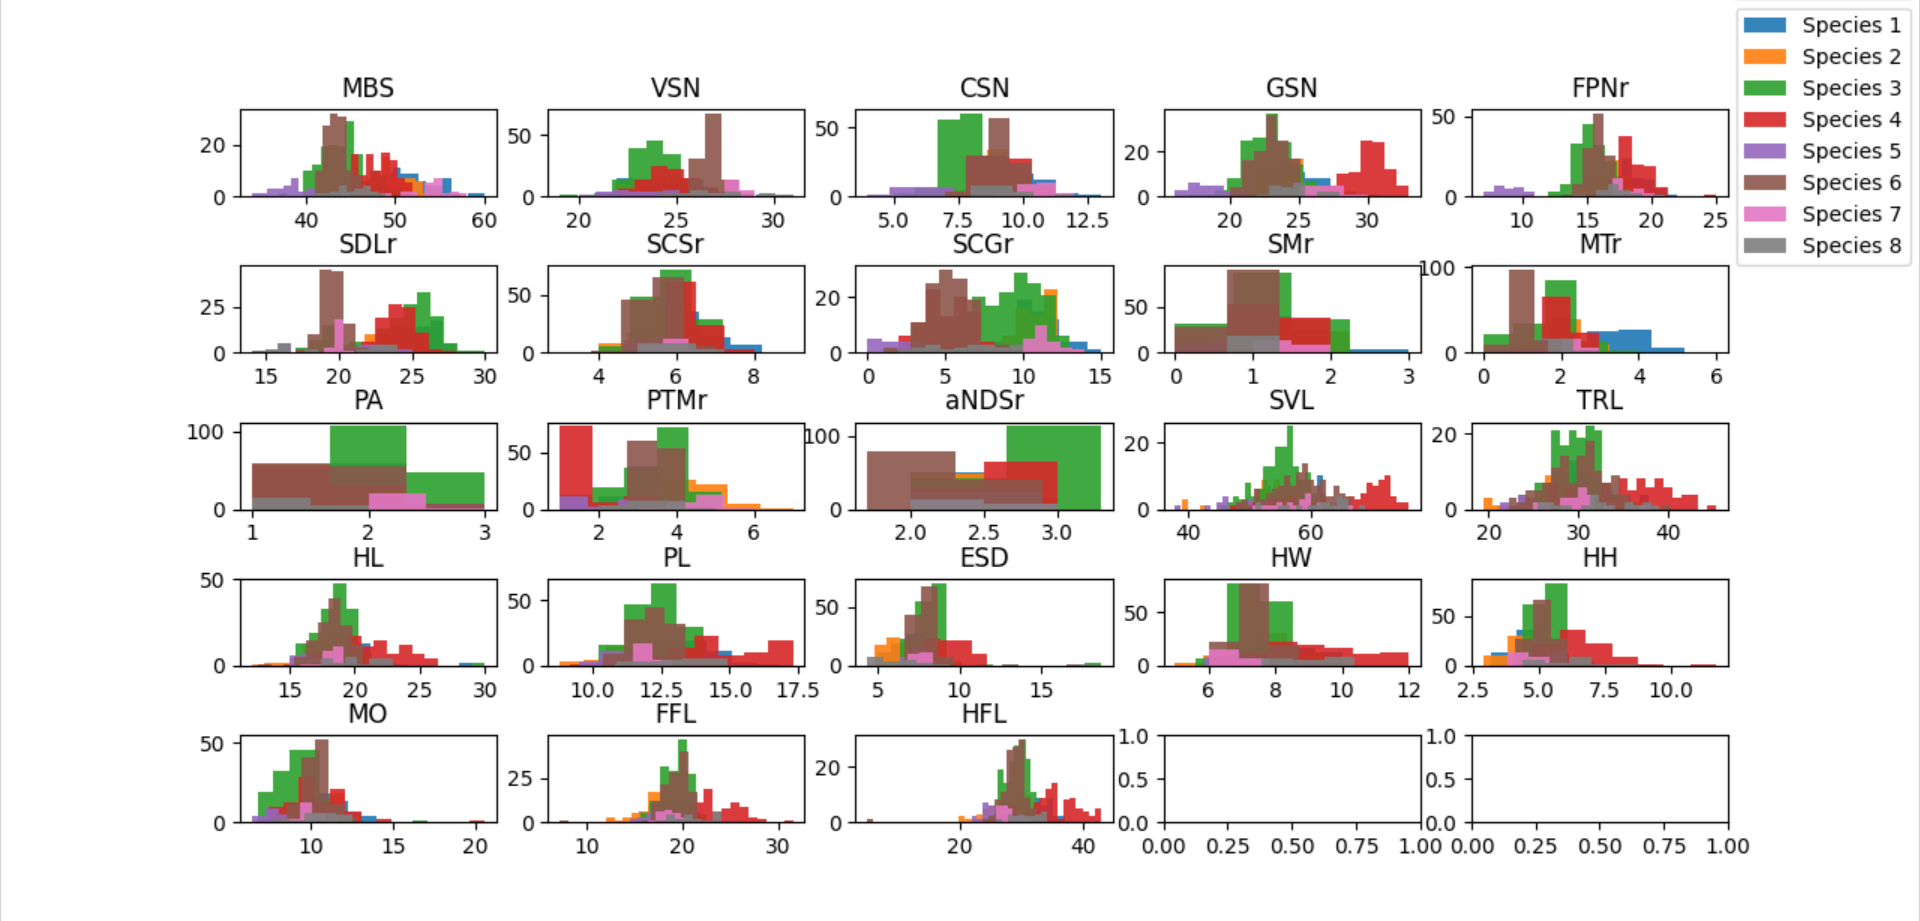
\includegraphics[scale=0.44]{fig1} \\
			\textit{Fig[1]: feature value histogram with regard to different species}
		\end{center}
		
		\begin{center}
			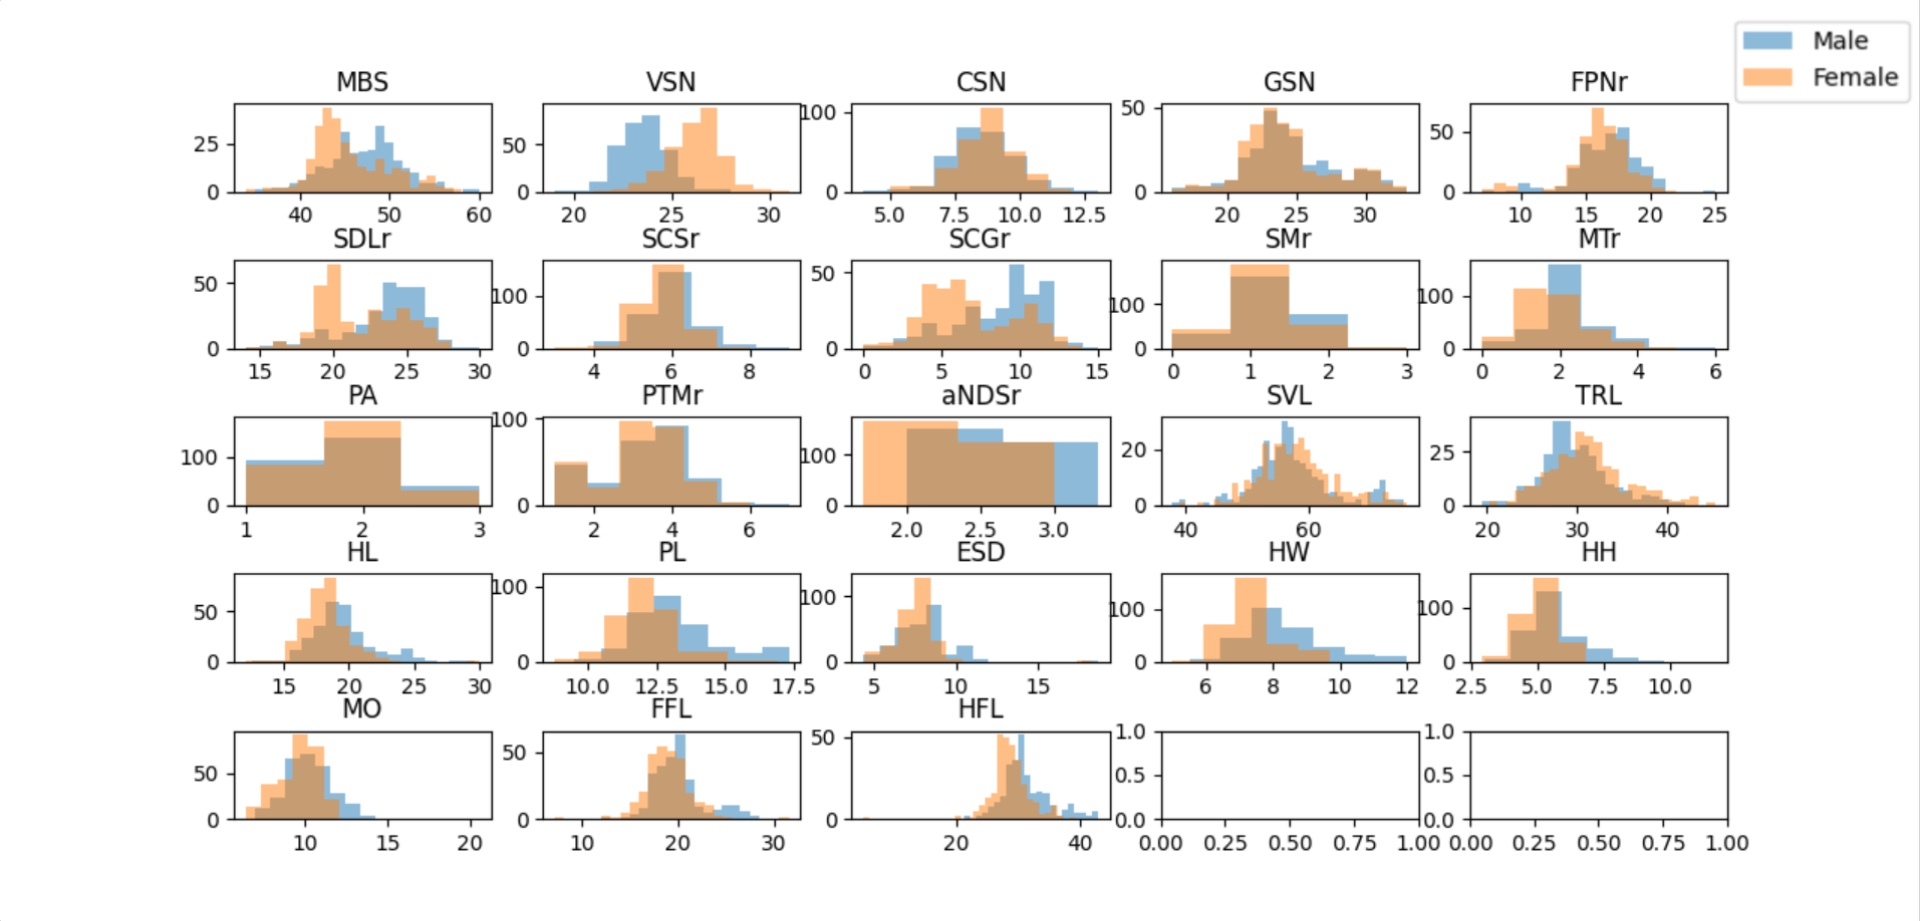
\includegraphics[scale=0.22]{fig2} \\
			\textit{Fig[2]: gender histogram with regard to different species}
		\end{center}
		
		Here we find the value of FNPr of species 5 is way smaller than others
		
		\begin{center}
			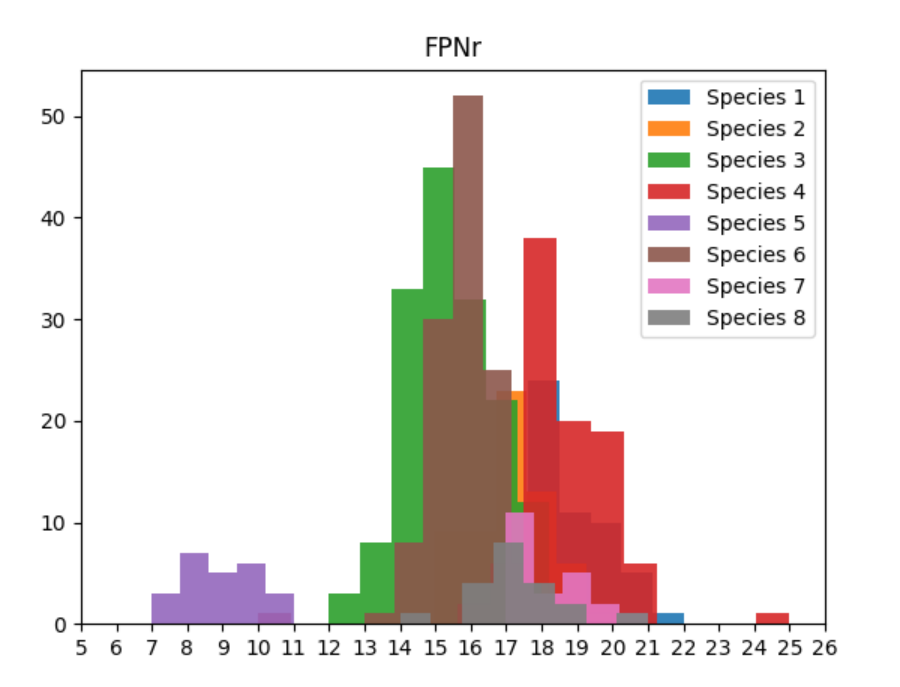
\includegraphics[scale=0.7]{fig3} \\
			\textit{Fig[3]: FNPr histogram with regard to different species}
		\end{center}
		
		\noindent Where all FNPr value of speces 5 is no greater than 11.
				
		Based on this phenomenon we observed, hence
		
		\begin{classifier}
			\begin{equation*}
				(classify(C) \stackrel{?}{=} 5) =
				\begin{cases}
					1 & C_4 \leq 11 \\
					0 & C_4 > 11
				\end{cases}
			\end{equation*}
		\end{classifier}
	
	\subsection{Parameterizing the Distributions}
		
		The data visualization shows us the distributions of $C_m \mid C \in S_n$ is roughly a
		Gaussian Distribution. So that we assume
		$$p(C_m \mid C \in S_n) \sim \mathcal{N}(\mu_{n, m}, \sigma_{n, m}^2)$$
		
		To check if this assumption fits the dataset, we calculated the kurtosis and skewness of it using Excel.
		
		$$Median \, of \, kurtosis = 3.04596$$
		$$Median \, of \, skewness = 0.05113$$
		
		Where Gaussian Distribution have a kurtosis of 3, and skewness of 0.
		This shows that for most $m$, $n$, $C_m \mid C \in S_n$ follows Gaussian Distribution.
	
	\subsection{Probability Model}
		
		Considering the probability of the Species\_num of a unclassified lizard $C$ equal to $n$,
		which is the expression below:
		
		$$p(C \in S_n \mid C_1, C_2, ..., C_{23})$$
		
		\noindent we have this classifier spontaneously
		
		\begin{classifier}
			$$classify(C)=\underset{i}{argmax}(p(C \in S_i \mid C_1, C_2, ..., C_{23}))$$
		\end{classifier}
		
		\noindent which means the Species\_num of unclassified lizard $C$ is $n$ such that
		the probability of $C \in S_n$ is the maximum.
		
		But we need to know the value of $p(C \in S_n \mid C_1, C_2, ..., C_{23})$ first.
		So we will try to use known conditions to calculate it.
		
		The derivation progress as below:
		
		\begin{lemma}[Bayes Theorem]
			$$p(A \mid B) = \dfrac{p(B \mid A)p(A)}{p(B)}$$
		\end{lemma}
		
		\begin{align*}
			  p(C \in S_n \mid C_1, C_2, ..., C_{23})
			&=\dfrac{p(C_1, C_2, ..., C_{23} \mid C \in S_n)p(C \in S_n)}{p(C_1, C_2, ..., C_{23})} \\
			&=\textcolor{blue}{\dfrac{p(C \in S_n, C_1, C_2, ..., C_{23})}{\sum^8_{i=1} p(C \in S_i, C_1, C_2, ..., C_{23})}}
		\end{align*}
		
		\noindent where
		
		\begin{align*}
			&\quad \ p(C \in S_n, C_1, C_2, ..., C_{23}) \\
			&=p(C \in S_n)p(C_1, C_2, ..., C_{23} \mid C \in S_n) \\
			&=p(C \in S_n)p(C_1 \mid C \in S_n)p(C_2, C_3, ..., C_{23} \mid C \in S_n, C_1) \\
			&=p(C \in S_n)p(C_1 \mid C \in S_n)p(C_2 \mid C \in S_n, C_1)p(C_3, C_4, ..., C_{23} \mid C \in S_n, C_1, C_2) \\
			&=... \\
			&=p(C \in S_n)p(C_1 \mid C \in S_n)...p(C_{23} \mid C \in S_n, C_1, C_2, ..., C_{22})
		\end{align*}
		
		\noindent since $C_i$ is independent of $C_j$ for $i \neq j$,
		
		\begin{align*}
			&\quad \ p(C \in S_n)p(C_1 \mid C \in S_n)...p(C_{23} \mid C \in S_n, C_1, C_2, ..., C_{22}) \\
			&=p(C \in S_n)p(C_1 \mid C \in S_n)p(C_2 \mid C \in S_n)p(C_3 \mid C \in S_n)...p(C_{23} \mid C \in S_n) \\
			&=\textcolor{blue}{p(C \in S_n)\prod_{i=1}^{23}p(C_i \mid C \in S_n)}
		\end{align*}
		
		\noindent also we knew
		
		$$p(C \in S_n) = f_n$$
		
		\noindent and
		
		$$C_i \mid C \in S_n \sim \mathcal{N}(\mu_{n, m}, \sigma_{n, m}^2)$$
		$$p(C_i \mid C \in S_n)=\dfrac{1}{\sigma_{n, m}\sqrt{2\pi}}e^{-\dfrac{(C_i-\mu_{n, m})^2}{2\sigma_{n, m}^2}}$$
		
		\noindent substitute these into \textcolor{blue}{these expression},
		we can calculate the value of
		$p(C \in S_n, C_1, C_2, ..., C_{23})$ and $p(C \in S_n \mid C_1, C_2, ..., C_{23})$
		
		Now, we managed to calculate all the variables in $classify(C)$, so we can
		classify lizards with this probability model.
		
		With the similar concept, we have
		
		\begin{classifier}
			$$gender(C)=\underset{i}{argmax}(P(C \in G_n \mid C_1, C_2, ..., C_{23}))$$
			where
			$$p(C \in G_n \mid C_1, C_2, ..., C_{23})
			= \dfrac{p(C \in G_n) \prod_{i = 1}^{23} p(C_i \mid C \in G_n)}{\sum_{k = 1}^2
			p(C \in G_k) \prod_{i = 1}^{23} p(C_i \mid C \in G_k)}$$
		\end{classifier}
		
		\noindent for the gender classification.
		
	\subsection{Model Optimization: Simplify}
		
		Considering a set of feature class $z$, after calculating similarly as before,
		
		$$p(C \in S_n \mid z) = \dfrac{p(C \in S_n)\prod_{k \in Z}p(k \mid C \in S_n)}{\sum_{i = 1}^8 p(C \in S_i)\prod_{k \in Z}p(k \mid C \in S_i)}$$
		
		\begin{classifier}
			$$classify(C) = \underset{i}{argmax}(p(C \in S_i \mid z))$$
		\end{classifier}
		
		If we are not considering all of the features, we need to find the $z$ that
		makes the accuracy this classifier as big as possible.
		
		So we can only consider about $p(C \in S_n \mid z)$.
		
		After reducing the conditions need to consider, the conditions left are 
		the differences between $S_n$ and other types of lizard.
	
	\newpage
	\section{Subproblem Solutions}
		\subsection{Subproblem 1}
		
			We have mentioned \textbf{Classfier 1}, which is designed for this
			subproblem.
				
			We have tested the accuracy of this classifier using the dataset given.
				
			\begin{center}
				\begin{tabular}{| c | c | c |}
				\hline
				& True species \#5 & True species \#1-4, 6-8 \\
				\hline
				Classified as species \#5 & 21 / 100\% & 1 / 0.19\% \\
				\hline
				Classified as species \#1-4, 6-8 & 0 / 0.0\% & 539 / 99.81\% \\
				\hline
				\end{tabular} \\
				\vspace{3mm}
				\textit{Table[1]: test result of Classifier 1}
			\end{center}
			
			This classifier is pretty good because it only classifies one lizard
			wrongly.
		
		\subsection{Subproblem 2}
			
			In subproblem 2, we need to find a set of feature class $z, |z|=2$ that makes
			$p(C \in S_5 \mid z)$ as large as possible.
			
			With help of computer, we found that when $z=\{C_1, C_5\}$, the accuracy of
			\textbf{Classifier 4} is the maximum possible.
			
			We have tested the accuracy and the results as shown down:
				
			\begin{center}
				\begin{tabular}{| c | c | c |}
				\hline
				& True species \#5 & True species \#1-4, 6-8 \\
				\hline
				Classified as species \#5 & 21 / 100\% & 0 / 0.0\% \\
				\hline
				Classified as species \#1-4, 6-8 & 0 / 0.0\% & 539 / 100.0\% \\
				\hline
				\end{tabular} \\
				\vspace{3mm}
				\textit{Table[2]: test result of Classifier 4 with $z=\{C_1, C_5\}$}
			\end{center}
		
		\newpage
		\subsection{Subproblem 3}
			
			Using \textbf{Classifier 3}, we can solve this problem.
			
			Validation result of \textbf{Classifier 3}:
			
			\begin{center}
				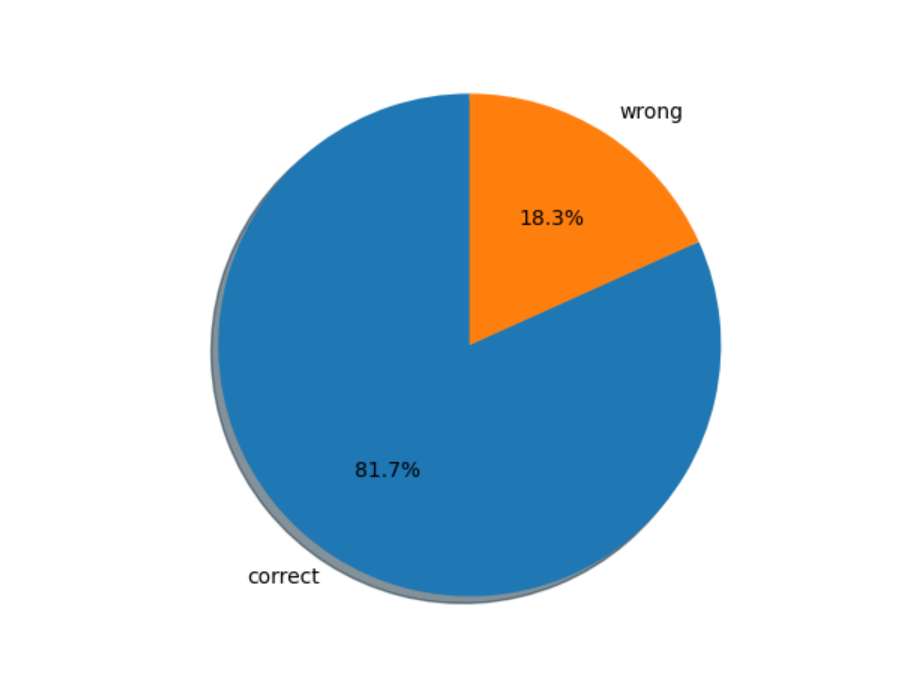
\includegraphics[scale=0.7]{fig5} \\
				\textit{Fig[4]: Accuracy of Classifier 3} \\
				\vspace{1cm}
				\begin{tabular}{||c||c|c||}
					\hline
					& Correctly Classified & Wrongly Classified \\
					\hline \hline
					Male & 212 (77.1\%) & 63 (22.9\%) \\
					\hline
					Female & 249 (86.2\%) & 40 (13.8\%) \\
					\hline
				\end{tabular} \\
				\vspace{3mm}
				\textit{Table[3]: Validation Result of Classifier 3}
			\end{center}
		
		\newpage
		\subsection{Subproblem 4}

			We can use \textbf{Classifier 2} to do the tasks of Subproblem 4.
			
			With help of Python, with packages \textit{Pandas}, \textit{NumPy},
			we validated \textbf{Classifier 2} using the dataset.
			
			\begin{center}
				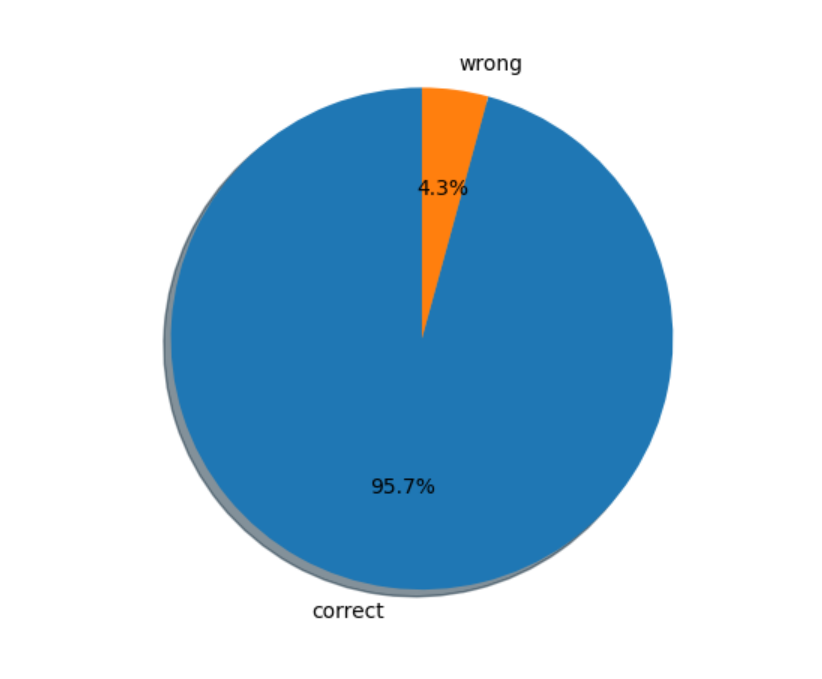
\includegraphics[scale=0.55]{fig4} \\
				\textit{Fig[5]: Accuracy of Classifier 2} \\
				\vspace{1cm}
				\begin{tabular}{||c||c|c||}
					\hline
					& Correctly Classified & Wrongly Classified \\
					\hline \hline
					Species 1 & 58 (87.9\%) & 8 (12.1\%) \\
					\hline
					Species 2 & 60 (95.2\%) & 3 (4.8\%) \\
					\hline
					Species 3 & 150 (96.2\%) & 6 (3.8\%) \\
					\hline
					Species 4 & 90 (96.8\%) & 3 (3.2\%) \\
					\hline
					Species 5 & 24 (100.0\%) & 0 (0.0\%) \\
					\hline
					Species 6 & 117 (97.5\%) & 3 (2.5\%) \\
					\hline
					Species 7 & 22 (100.0\%) & 0 (0.0\%) \\
					\hline
					Species 8 & 19 (95.0\%) & 1 (5\%) \\
					\hline
				\end{tabular} \\
				\vspace{3mm}
				\textit{Table[4]: Accuracy of Classifier 2 for each species}
			\end{center}
			
			From the perspective of the correct classification probability of a single species, we notice that although the correct rate of species one is the lowest, the correct classification is close to 90\%(87.5\%), followed by species 2, 3, 4 and 8, and the correct rates are all around ninety-five percent, respectively 95.2\%, 96.2\%, 96.8\% and 95\%. Compare to the species 6, the correct rate is nearly one-hundred percent (97.5 \%).  It is worth noting that the classification accuracy rate of species 5 and 7 reached 100\%, which means the classification is completely correct. So we think that the criteria that we have established are applicable to task four.
			
		\subsection{Subproblem 5}
			For subproblem 5, we can use \textbf{Classifier 2} and \textbf{Classifier 3},
			which are mentioned on the solution of previous subproblems.
			We validated the accuracy of using \textbf{Classifier 2} and \textbf{Classifier 3}
			at the same time.
			
			\begin{center}
				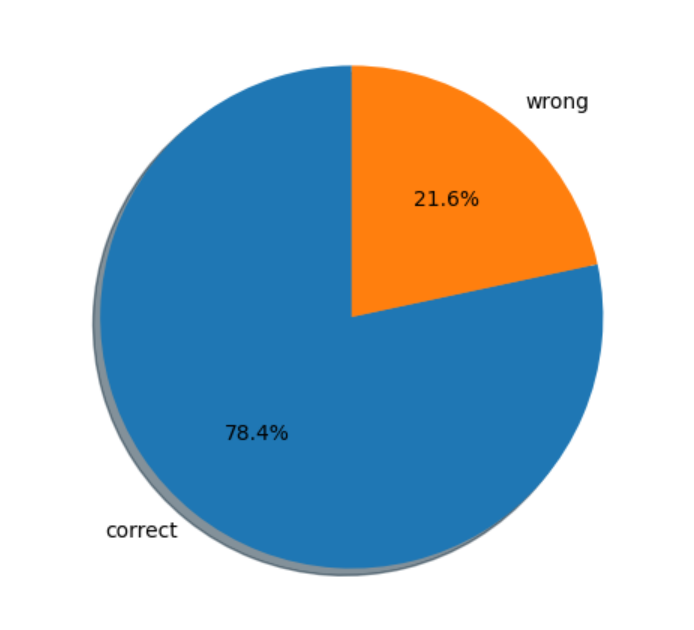
\includegraphics[scale=0.8]{fig6} \\
				\textit{Fig[6]: Accuracy of using Classifier 2 and Classifier 3 together}
				\vspace{3mm}
			\end{center}
			
			\noindent which we can see that this accuracy is slightly lower than only using
			\textbf{Classifier 3}
	
	\newpage
	\section{Result Analysis}
		\subsection{Strengths}
			\begin{itemize}
				\item
				\textbf{Efficiency in updating data} \\
				When more data is added to the object we want to study, the probability algorithm can update the results at a higher speed. Even for very large-scale data sets, each item usually only corresponds to an individual feature number.  So our selected model has stable classification efficiency.
				\item
				\textbf{Simplicity of algorithms and ease of interpretation of results} \\
				This probability algorithm does not need to use complex computer program calculations, but only needs to use basic mathematical operations to solve it.  Moreover, the required calculation time is shorter, the algorithm logic is simple and stable, and the interpretation of the results is easier to understand.
			\end{itemize}
		
		\subsection{Weakness}
			\begin{itemize}
				\item
				\textbf{The deviation of value} \\
					Through the chart of Task 1 and the calculation of Kurtosis and skewness, we determines that the data we studied conformed to the Gaussian distribution. But from the final results, our data still differs from the Gaussian distribution image. As a result, the classification cannot be exactly close to 100%.
				\item
				\textbf{Sample correlation can have an impact} \\
					In order to ensure the best classification effect, we assume that there is independence between samples. But in reality, there will inevitably be inextricable relationships between many data.This means that the data cannot be completely independent of each other, which let  the Naive Bayes algorithm is not applicable at this time.
			\end{itemize}
		
		\subsection{Expectation}
			\begin{itemize}
				\item
				\textbf{Parameterize the distributions using Gaussian Mixture Model, instead of single Gaussian Distribution} \\
				Because not all of the distribution follows Gaussian Distribution, this deviation
				make the accuracy of our gender classifier low. If we Parameterize the distributions
				using Gaussian Mixture Model, we can get a better accuracy on our gender classifier
				
			\end{itemize}

\newpage
\thispagestyle{plain}
\pagenumbering{roman}
\begin{thebibliography}{9}
\bibitem{Darevskia}
Bo Beolens, Michael Watkins, Michael Grayson(2011).
The Eponym Dictionary of Reptiles.
Baltimore: Johns Hopkins University Press.
\end{thebibliography}

\newpage
\thispagestyle{plain}
\section*{Appendix}
\hypertarget{tab:feature}{}
\textbf{Feature index table} \\
\begin{center}
	\begin{tabular}{||c|c||c|c||}
		\hline
		Feature name & index & Feature name & index \\
		\hline
		MBS & 1 & aNDSr & 13 \\
		\hline
		VSN & 2 & SVL & 14 \\
		\hline
		CSN & 3 & TPL & 15 \\
		\hline
		GSN & 4 & HL & 16 \\
		\hline
		FPNr & 5 & PL & 17 \\
		\hline
		SDLr & 6 & ESD & 18 \\
		\hline
		SCSr & 7 & HW & 19 \\
		\hline
		SCGr & 8 & HH & 20 \\
		\hline
		SMr & 9 & MO & 21 \\
		\hline
		MTr & 10 & FFL & 22 \\
		\hline
		PA & 11 & HFL & 23 \\
		\hline
		PTMr & 12 & & \\
		\hline
	\end{tabular}
\end{center}
\subsection*{Classification Code}
\begin{lstlisting}[language=Python]
#!/usr/bin/env python3
import numpy as np
import math
import pandas as pd


df = pd.read_excel("dataset.xlsx")


species_mean = [df[df["Species_num"] == i + 1].iloc[:, 3:].mean() for i in range(8)]
species_std = [df[df["Species_num"] == i + 1].iloc[:, 3:].std() for i in range(8)]
species_density = df["Species_num"].value_counts(normalize=True)

gender_mean = [df[df["Sex_num"] == i + 1].iloc[:, 3:].mean() for i in range(3)]
gender_std = [df[df["Sex_num"] == i + 1].iloc[:, 3:].std() for i in range(3)]
gender_density = df["Sex_num"].value_counts(normalize=True)


def gaussian(mean, std, x):
    if math.isnan(mean) or math.isnan(std):
        return 0
    return 1 / (std * (2 * math.pi) ** 0.5) * math.exp(-(x - mean) ** 2 / (2 * std ** 2))


def classifier2(feat):
    prob = [species_density[i] for i in range(1, 9)]
    for i in range(8):
        for j in range(23):
            prob[i] *= gaussian(species_mean[i][j], species_std[i][j], feat[j])
    prob /= sum(prob)
    return np.argmax(prob)


def classifier3(feat):
    prob = [gender_density[i] for i in range(1, 3)]
    for i in range(2):
        for j in range(23):
            prob[i] *= gaussian(gender_mean[i][j], gender_std[i][j], feat[j])
    prob /= sum(prob)
    return np.argmax(prob)


correct_species = 0
wrong_species = 0
correct_gender = 0
wrong_gender = 0
correct = 0
wrong = 0

for i in range(len(df)):
    feat = df.iloc[i, 3:]
    species = classifier2(feat)
    gender = classifier3(feat)
    if species + 1 == df["Species_num"][i]:
        correct_species += 1
    else:
        wrong_species += 1
    if gender + 1 == df["Sex_num"][i]:
        correct_gender += 1
    else:
        wrong_gender += 1
    if gender + 1 == df["Sex_num"][i] and species + 1 == df["Species_num"][i]:
        correct += 1
    else:
        wrong += 1

print(correct / (correct + wrong), wrong / (correct + wrong))
\end{lstlisting}

\end{document}